Having some metrics to compare the articles between years, we thought it was a good idea to try to date a subset of articles from a year with these metrics. Thus, we wrote a \emph{Scala} application that selects a subset of articles in a year and we considered this subset of articles as a year to be able to reuse the same code as for the comparison between years. Nevertheless, we had to adapt a bit our codes because it was unnecessary to compare years with years but only articles with years. We also had to remove the articles from the year they belong to. Finally, we selected a subset of articles and not only one article because in the corpus, some titles of articles in the newspaper are considered as a complete article. Thus, it has no sense to have the possibility to select only one article with 4 or 5 words.\\

You can find below the different results for the different metrics with the years 1880, 1920 and 1995 and with taking 15 articles in each year.

\subsection{Metrics}

\subsubsection{Basic Distance}
Here are some example where the distance is applied between the selected subset of articles and each year of the corpus:
\begin{figure}[H]
    \begin{minipage}[b]{0.3\linewidth}
        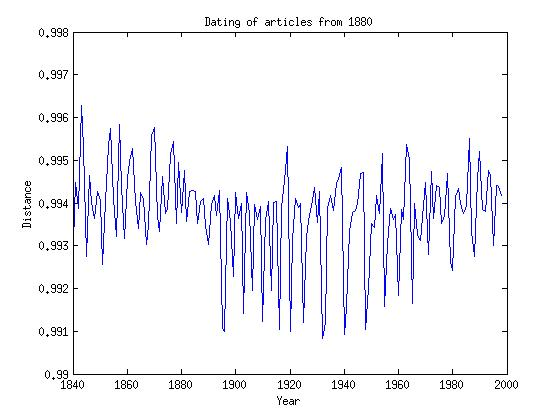
\includegraphics[scale=0.25]{Pictures/date_articles/distance1/dating1880.jpg}
        \caption{Dating articles from 1880 with the basic distance. Prediction is 1932.}
    \end{minipage}\hfill
    \begin{minipage}[b]{0.3\linewidth}
        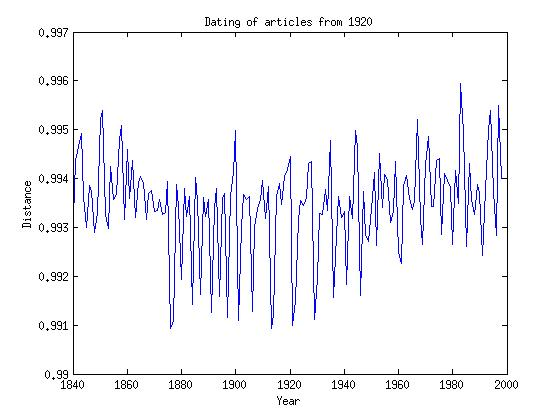
\includegraphics[scale=0.25]{Pictures/date_articles/distance1/dating1920.jpg}
        \caption{Dating articles from 1920 with the basic distance. Prediction is 1913.}
    \end{minipage}\hfill
    \begin{minipage}[b]{0.3\linewidth}
	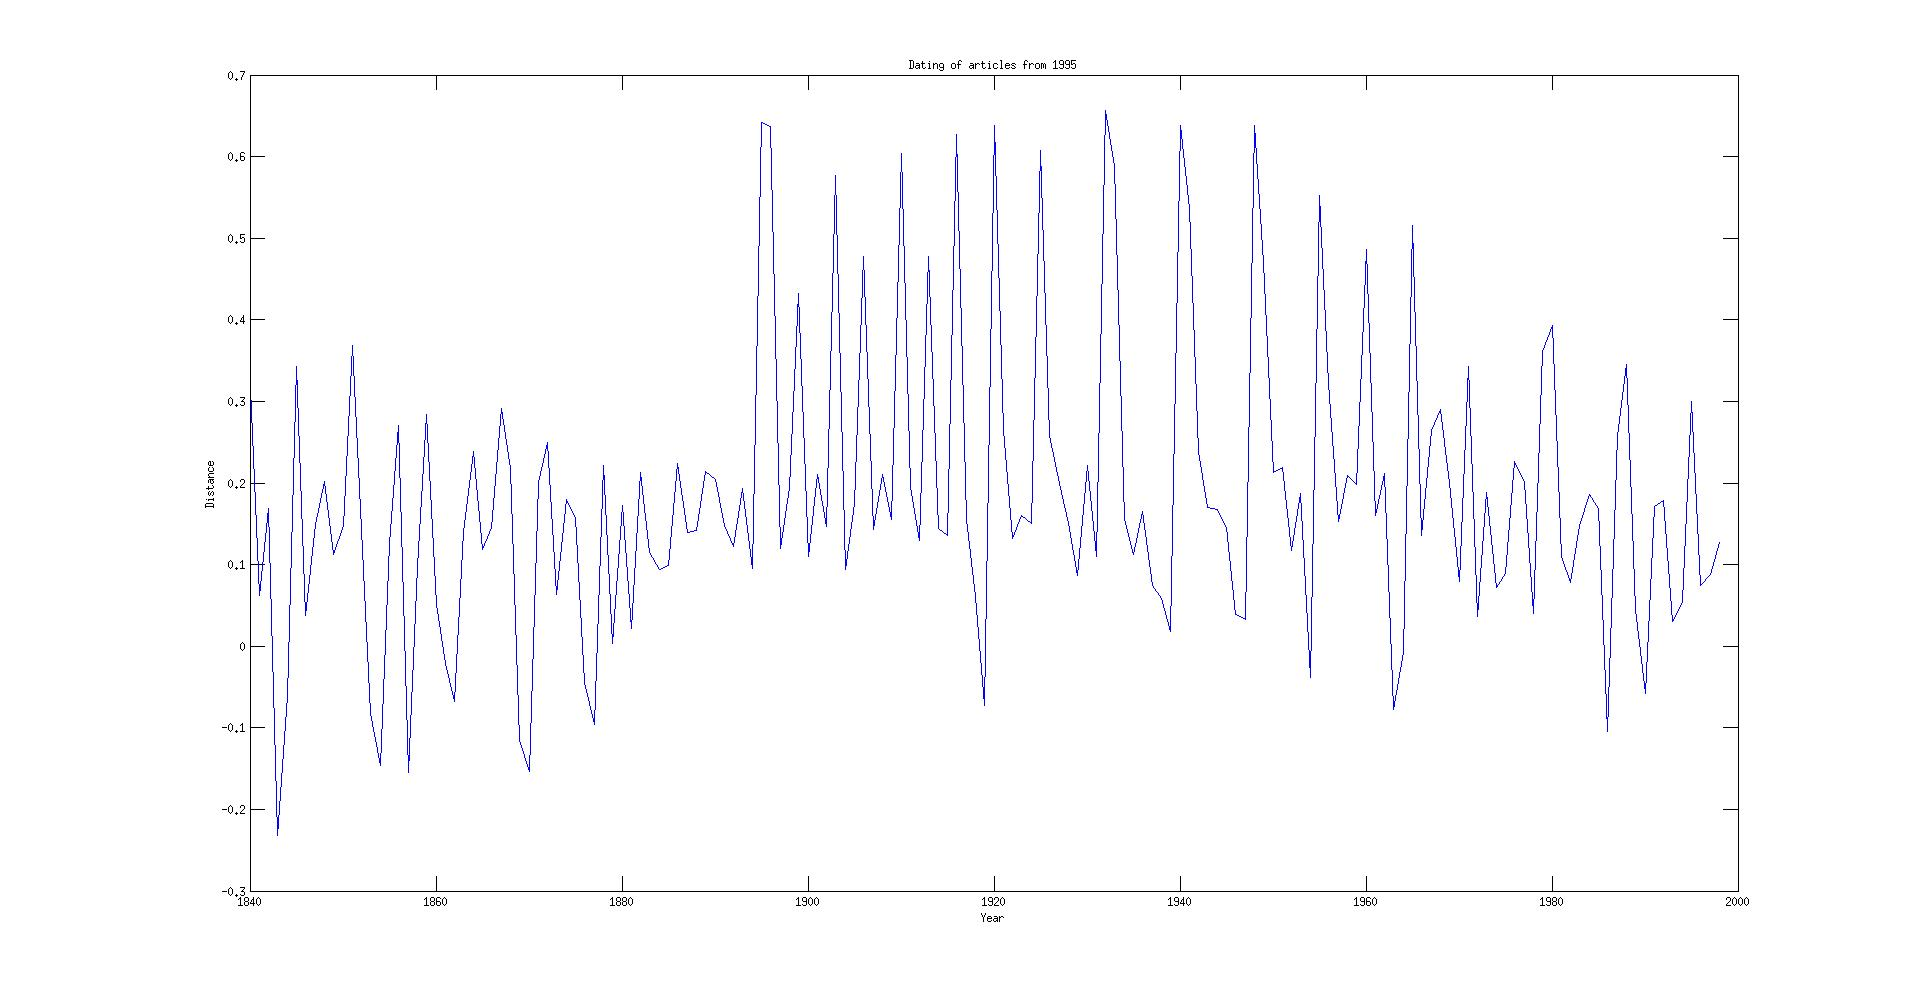
\includegraphics[scale=0.25]{Pictures/date_articles/distance1/dating1995_corrected.jpg}
        \caption{Dating articles from 1995 with the basic distance. Prediction is 1843.}
    \end{minipage}
\end{figure}
With the basic metric, the distances look very random, and the minimum doesn't give a good prediction. In our opinion, this "sawteeth" behavior can be explained because the amount of words suddenly drop in certain years. Indeed, the basic distance is subject to the number of words in each year and knowing that in 1840's years there are less words in the others and that between 1917 and 1919 and in 1998 there are less articles too, the predicted year will almost always one of the previous ones.

\subsubsection{Chi Square}
\begin{figure}[H]
	\centering
        \includegraphics[scale=0.15]{Pictures/date_articles/chi2/dating1995_corrected.jpg}
        \caption{Dating articles from 1995 with the chi-square distance}
        \label{date_chi2}
\end{figure}
With the chi-square distance, there is again no evident prediction in the example in figure \ref{date_chi2} where the prediction is 1858 for articles from 1995.
\subsubsection{Cosine}

\begin{figure}[H]
    \begin{minipage}[b]{0.3\linewidth}
        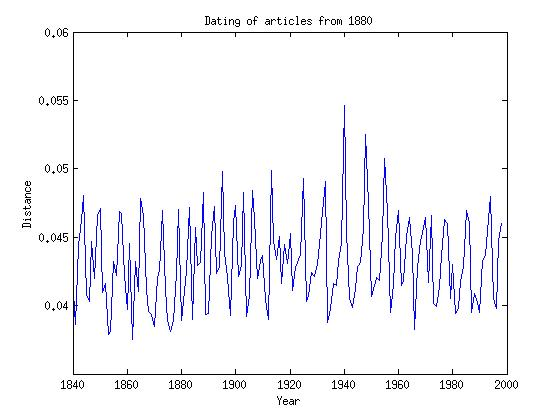
\includegraphics[scale=0.25]{Pictures/date_articles/cos/dating1880.jpg}
        \caption{Dating articles from 1880 with the cosine distance. Prediction is 1862.}
    \end{minipage}\hfill
    \begin{minipage}[b]{0.3\linewidth}
        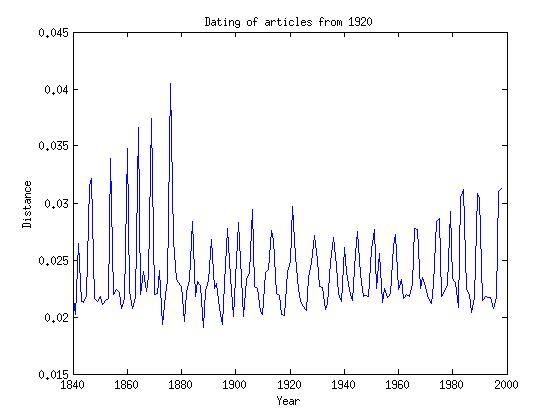
\includegraphics[scale=0.25]{Pictures/date_articles/cos/dating1920.jpg}
        \caption{Dating articles from 1920 with the cosine distance. Prediction is 1889.}
    \end{minipage}\hfill
    \begin{minipage}[b]{0.3\linewidth}
	\includegraphics[scale=0.25]{Pictures/date_articles/cos/dating1995_corrected.jpg}
        \caption{Dating articles from 1995 with the cosine distance. Prediction is 1866}
        \label{date_cos}
    \end{minipage}
\end{figure}
The cosine distance seems to have the same behaviour as the basic and \emph{Chi-Square} distances for dating. Its predictions are also not accurate.
\subsubsection{Cosine with TF-IDF}
\subsubsection{Kullback-Leibler Divergence}
Figures \ref{ArticleKL-C1880} to \ref{ArticleKL-N1995} show the results for the 3 different years trying to represent the articles with each year :

\begin{figure}[h!]
    \begin{minipage}[b]{0.48\linewidth}
        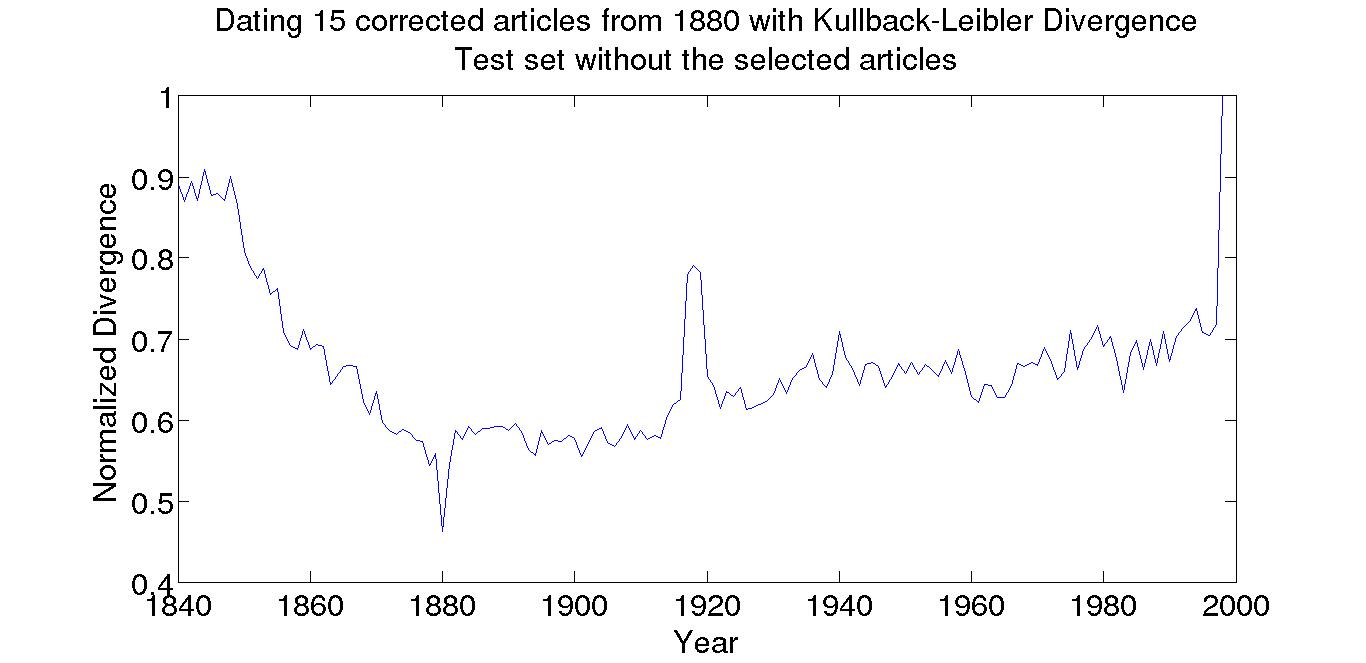
\includegraphics[scale=0.15]{Pictures/date_articles/kullback_leibler/15articles_1880_KL_years_simulate_articles_corrected_without_articles.jpg}
        \caption{KL for 15 articles with OCR correction for year 1880}
        \label{ArticleKL-C1880}
    \end{minipage}\hfill
    \begin{minipage}[b]{0.5\linewidth}
        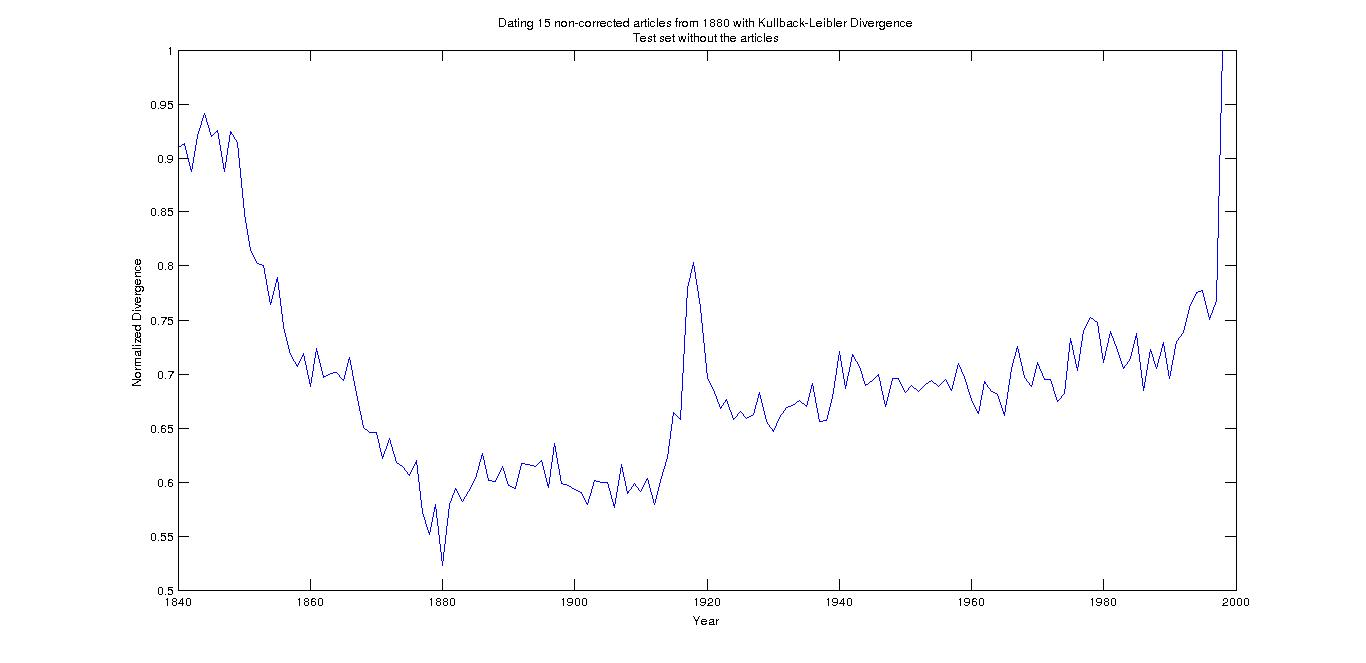
\includegraphics[scale=0.15]{Pictures/date_articles/kullback_leibler/15articles_1880_KL_years_simulate_articles_without_correction_without_articles.jpg}
        \caption{KL for 15 articles without OCR correction for year 1880}
        \label{ArticleKL-N1880}
    \end{minipage}\hfill
\end{figure}

\begin{figure}[h!]
    \begin{minipage}[b]{0.48\linewidth}
        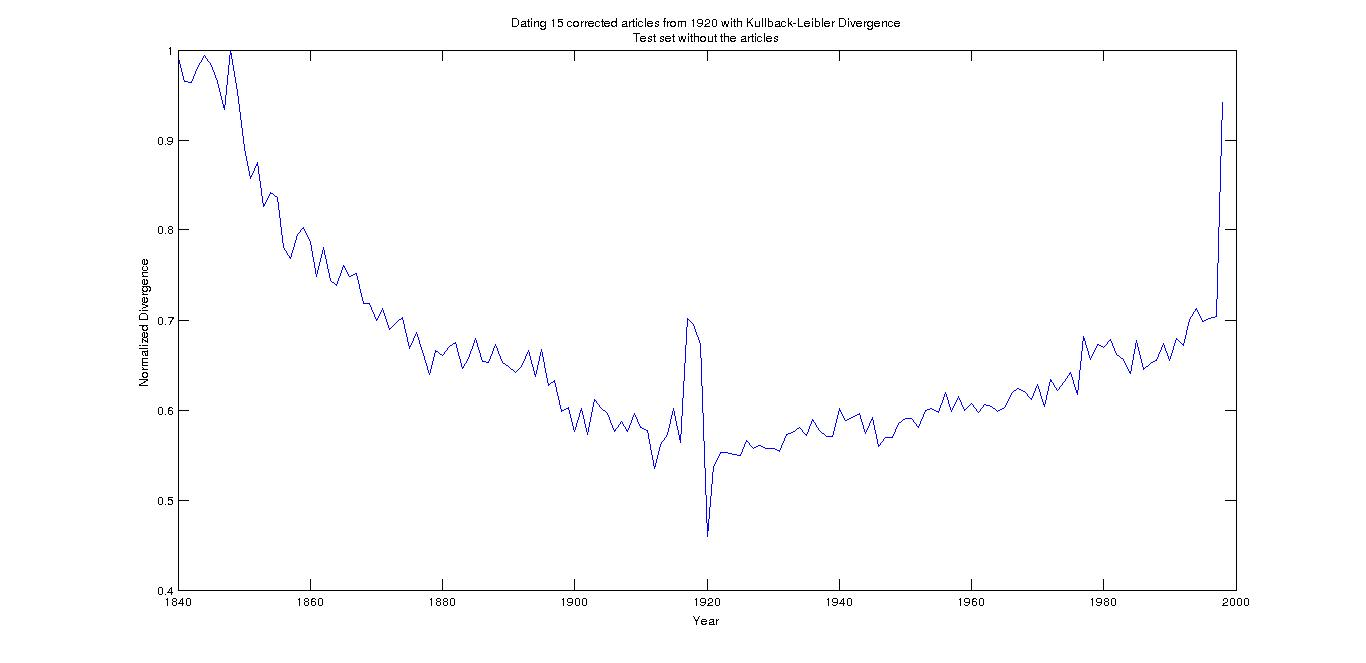
\includegraphics[scale=0.15]{Pictures/date_articles/kullback_leibler/15articles_1920_KL_years_simulate_articles_corrected_without_articles.jpg}
        \caption{KL for 15 articles with OCR correction for year 1920}
        \label{ArticleKL-C1920}
    \end{minipage}\hfill
    \begin{minipage}[b]{0.5\linewidth}
        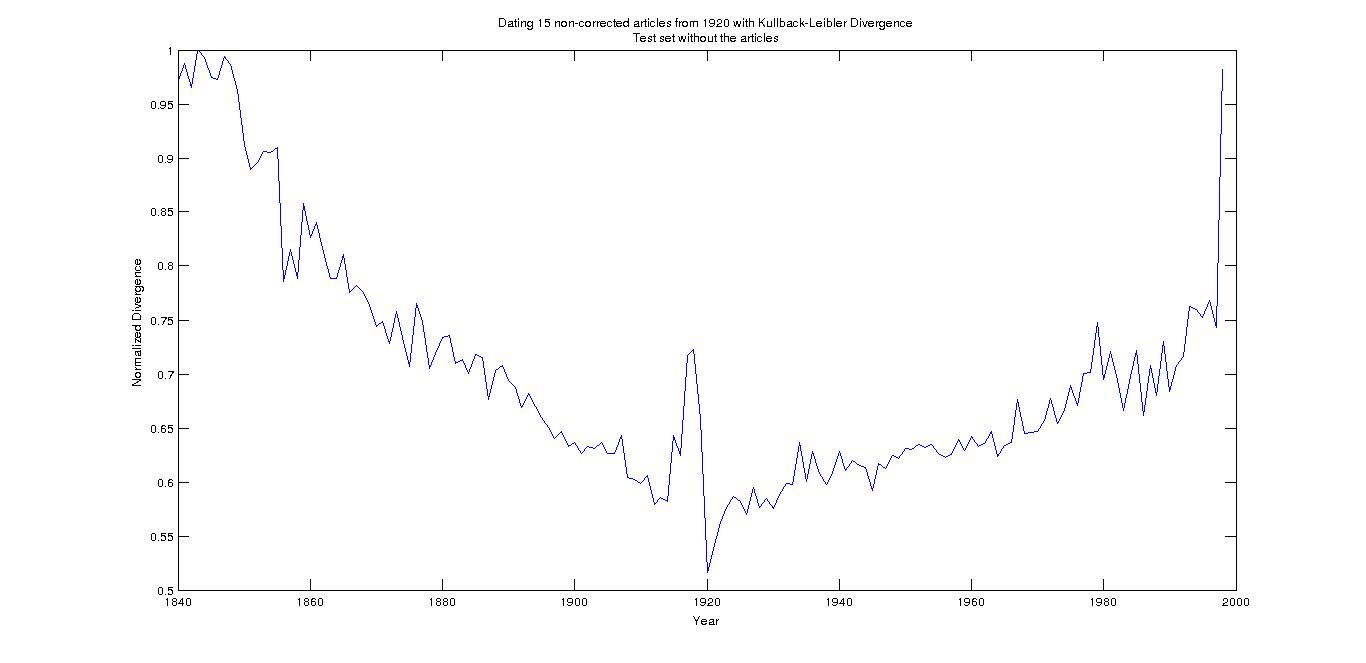
\includegraphics[scale=0.15]{Pictures/date_articles/kullback_leibler/15articles_1920_KL_years_simulate_articles_without_correction_without_articles.jpg}
        \caption{KL for 15 articles without OCR correction for year 1920}
        \label{ArticleKL-N1920}
    \end{minipage}\hfill
\end{figure}

\begin{figure}[h!]
    \begin{minipage}[b]{0.48\linewidth}
        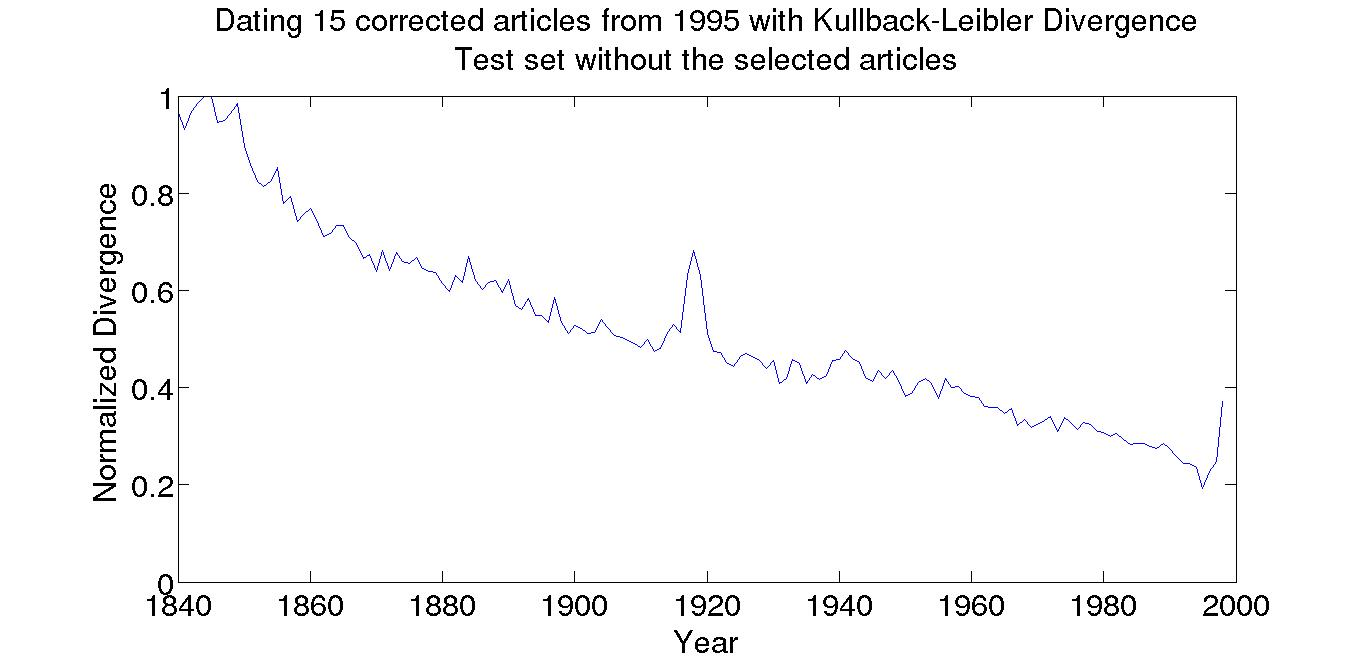
\includegraphics[scale=0.15]{Pictures/date_articles/kullback_leibler/15articles_1995_KL_years_simulate_articles_corrected_without_articles.jpg}
        \caption{KL for 15 articles with OCR correction for year 1995}
        \label{ArticleKL-C1995}
    \end{minipage}\hfill
    \begin{minipage}[b]{0.5\linewidth}
        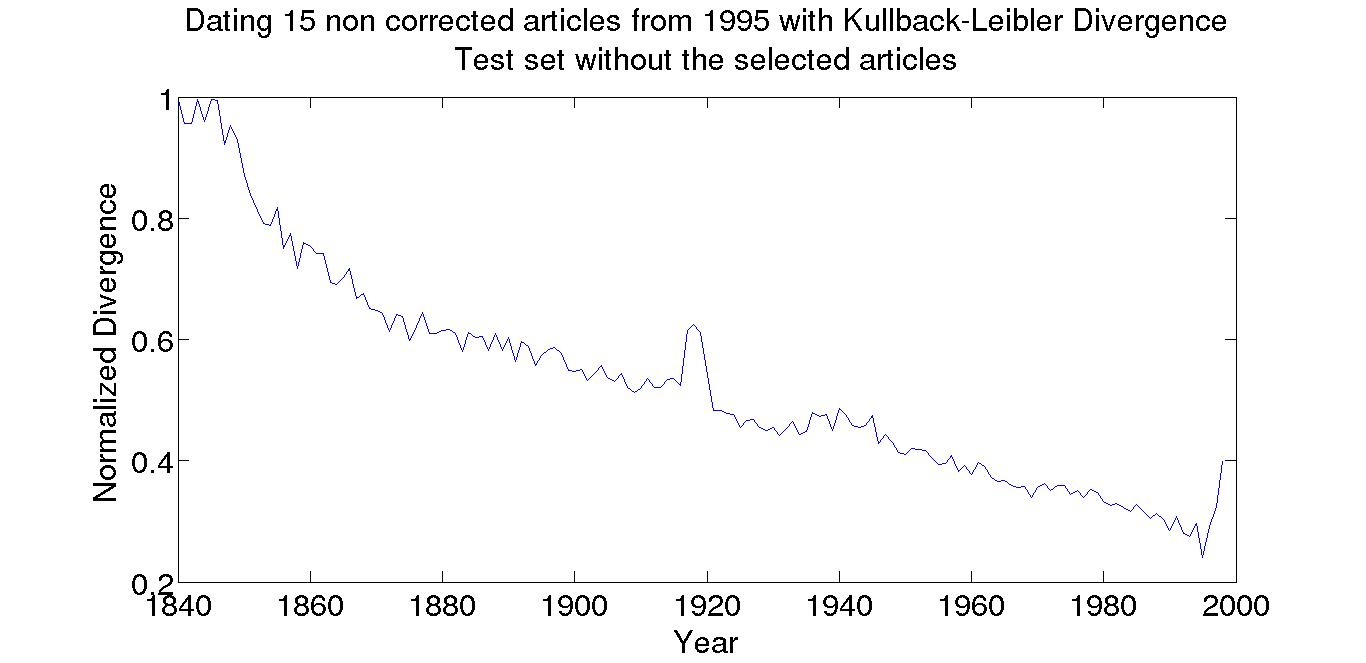
\includegraphics[scale=0.15]{Pictures/date_articles/kullback_leibler/15articles_1995_KL_years_simulate_articles_without_correction_without_articles.jpg}
        \caption{KL for 15 articles without OCR correction for year 1995}
        \label{ArticleKL-N1995}
    \end{minipage}\hfill
\end{figure}

We took only the direction where the year approximate the articles because it has no sense to do the inverse. Indeed, to approximate a year that contains thousands of words with a subset of articles that contains a few hundred words will lead to a dating that will very often predict the years with less words (in the 19$th$ century).

We can observe again in these figures that the OCR correction does not help so much for dating. But, we can observe that the \emph{Kullback-Leibler} Divergence is really good to date the articles. Our explanation for these excellent results is that when we remove some articles from a year, the probability that the words are present in this year is higher than in other years. So, even if we remove the articles from the year, it stays hardly attached to the article and when the year approximate the articles, it has a really good matching.

\subsubsection{Out of Place}
In this part, we using \emph{Out of Place} measurement to date the article by two different kind of approaches (i.e., whether use unmatched word or not). See figure \ref{outofplace_1840_all}, \ref{outofplace_1840_match},\ref{outofplace_1960_all}, \ref{outofplace_1960_match}, \ref{outofplace_1995_all} and \ref{outofplace_1995_match} for more details.

\begin{figure}[H]
    \begin{minipage}[b]{0.48\linewidth}
        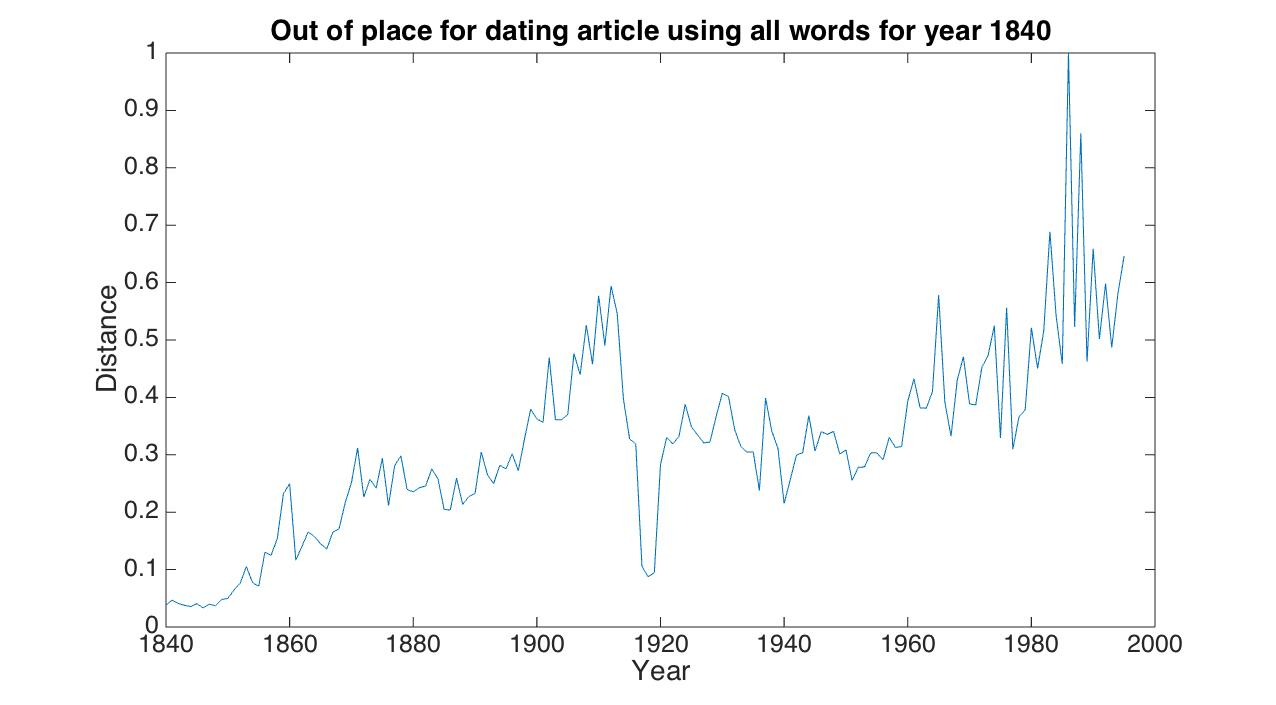
\includegraphics[scale=0.15]{Pictures/date_articles/outofplace/1840_all.jpg}
        \caption{Out of place for dating article using all words for year 1840}
        \label{outofplace_1840_all}
    \end{minipage}\hfill
    \begin{minipage}[b]{0.5\linewidth}
        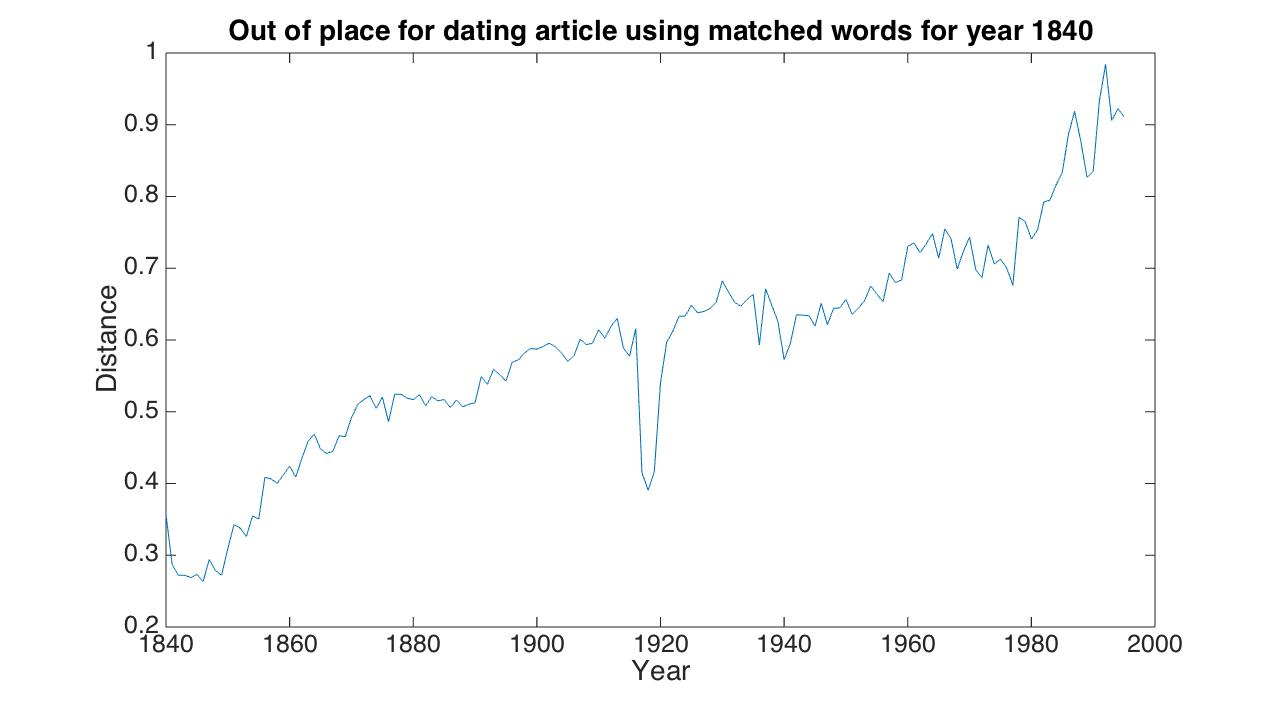
\includegraphics[scale=0.15]{Pictures/date_articles/outofplace/1840_partial.jpg}
        \caption{Out of place for dating article using matched words for year 1840}
        \label{outofplace_1840_match}
    \end{minipage}\hfill
\end{figure}

\begin{figure}[H]
    \begin{minipage}[b]{0.48\linewidth}
        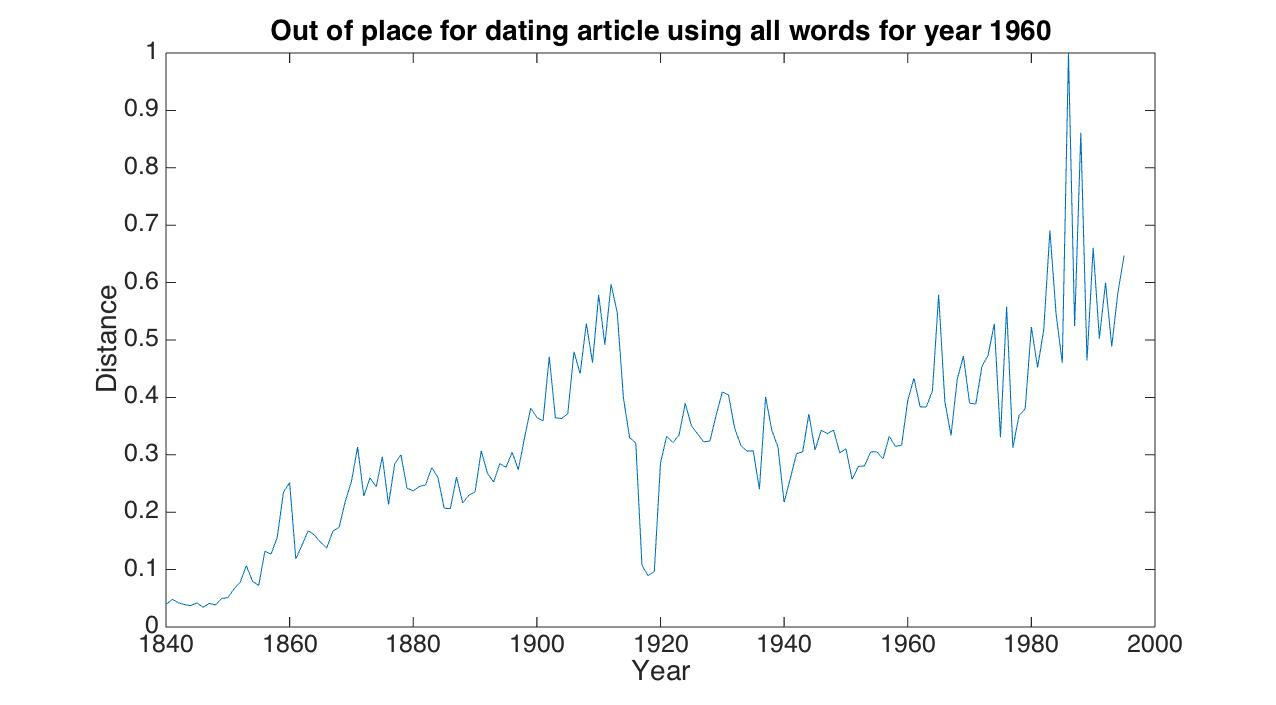
\includegraphics[scale=0.15]{Pictures/date_articles/outofplace/1960_all.jpg}
        \caption{Out of place for dating article using all words for year 1960}
        \label{outofplace_1960_all}
    \end{minipage}\hfill
    \begin{minipage}[b]{0.5\linewidth}
        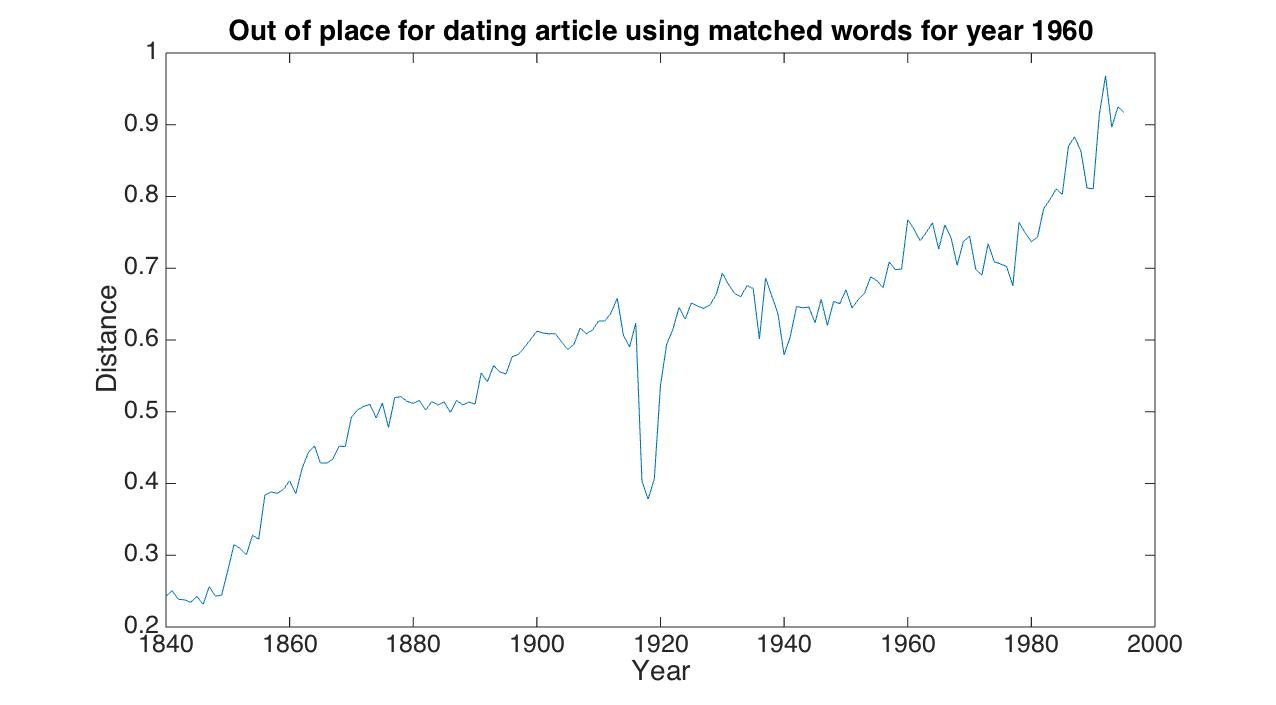
\includegraphics[scale=0.15]{Pictures/date_articles/outofplace/1960_partial.jpg}
        \caption{Out of place for dating article using matched words for year 1960}
        \label{outofplace_1960_match}
    \end{minipage}\hfill
\end{figure}

\begin{figure}[H]
    \begin{minipage}[b]{0.48\linewidth}
        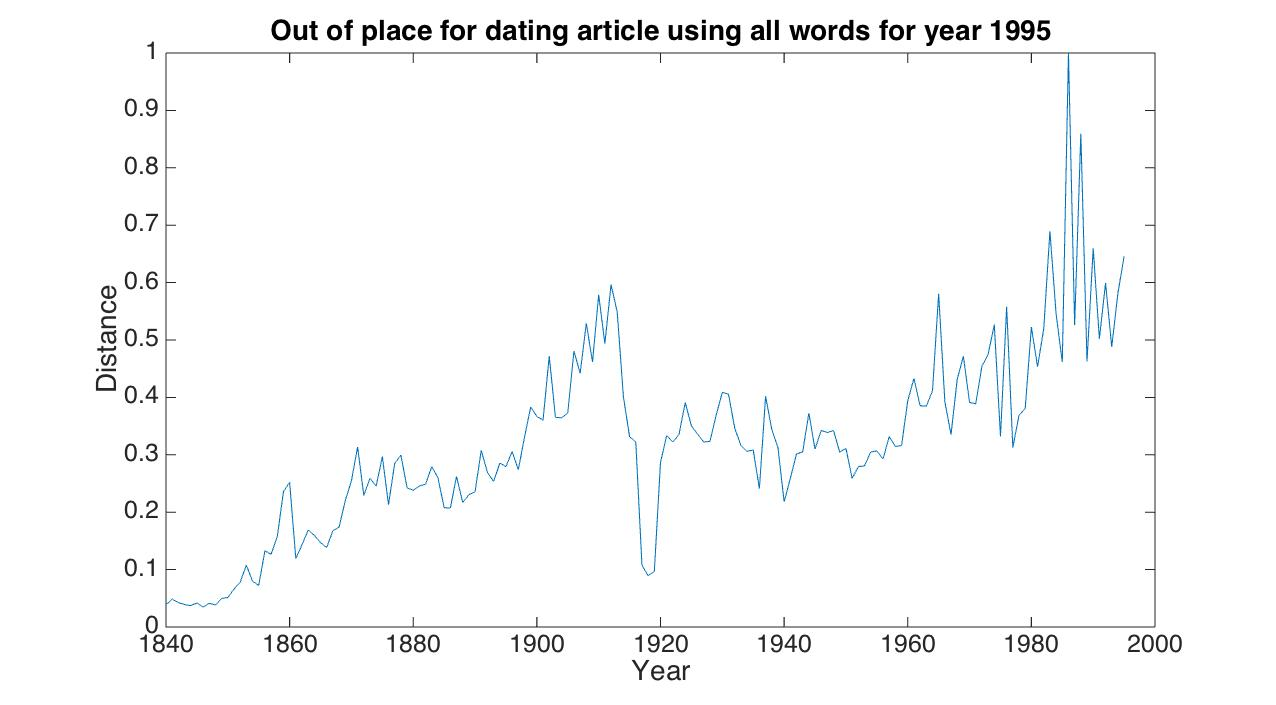
\includegraphics[scale=0.15]{Pictures/date_articles/outofplace/1995_all.jpg}
        \caption{Out of place for dating article using all words for year 1995}
        \label{outofplace_1995_all}
    \end{minipage}\hfill
    \begin{minipage}[b]{0.5\linewidth}
        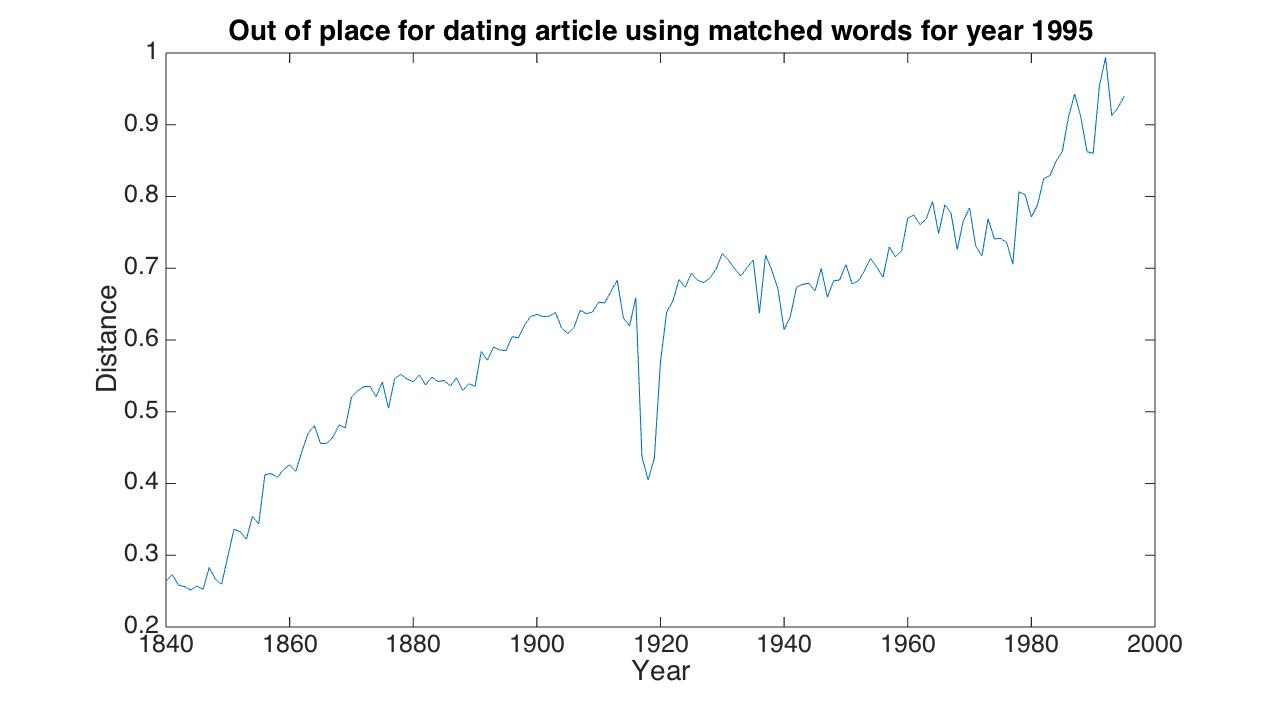
\includegraphics[scale=0.15]{Pictures/date_articles/outofplace/1995_partial.jpg}
        \caption{Out of place for dating article using matched words for year 1995}
        \label{outofplace_1995_match}
    \end{minipage}\hfill
\end{figure}

If we only look at the result of year $1840$, we can say that it is a good metric for its high-accuracy of prediction. However, when tracking the condition on other years, the result is really odd since all of them give a same plot if we just classify them by eyes. Check its detailed information, there exists a slight difference between different pairs of article and years for the \emph{Out of Place} measurement. However, we cannot deny that it works bad on dating article.

Returning to the formula of \emph{Out of Place} measurement and also considering the size of article, this odd phenomenon then can be explained. For dating article, we only randomly select 15 articles whose size is too small to affect the rank of words that appears in the year data even though we have already removed word's frequency of article from the year it belongs to. As a result, noises are introduced to the final result or useful information are missing.

If we use all words, due to the big gap between the size of article and years, valuable information will be hidden by large volume noises which explains the unchangeable phenomenon on the distance of different article and years. If we only use matched words, for articles that from different years, the matched words are greatly limited by the year data, thus the computation process will always happen on the similar article dataset and year dataset if article data varies but year data remains the same. That is why the \emph{Out of Place} measurement met some changes among part of relationships but still remain a similar trend.

Thus, as explained above, the \emph{Out of Place}, at least for the function of dating article, is not a good metric.


\subsubsection{Punctuation and sentences length}
As the statistics on punctuation and sentences tend to change between years (especially for the sentences lengths and number of commas), we tried to implement a metric with those statistics. \\

Those statistics are extracted for each year and combined in a single entry by year. For the metric, we take a sample of articles from one year, we merge them, as it was one big article, we compute the statistics on this article and we use a simple euclidean distance to compute the distance with each year. The result for a sample of 15 random articles from 1925 is observable in figure \ref{punct_metric_1925}.

\begin{figure}[H]
	\centering
    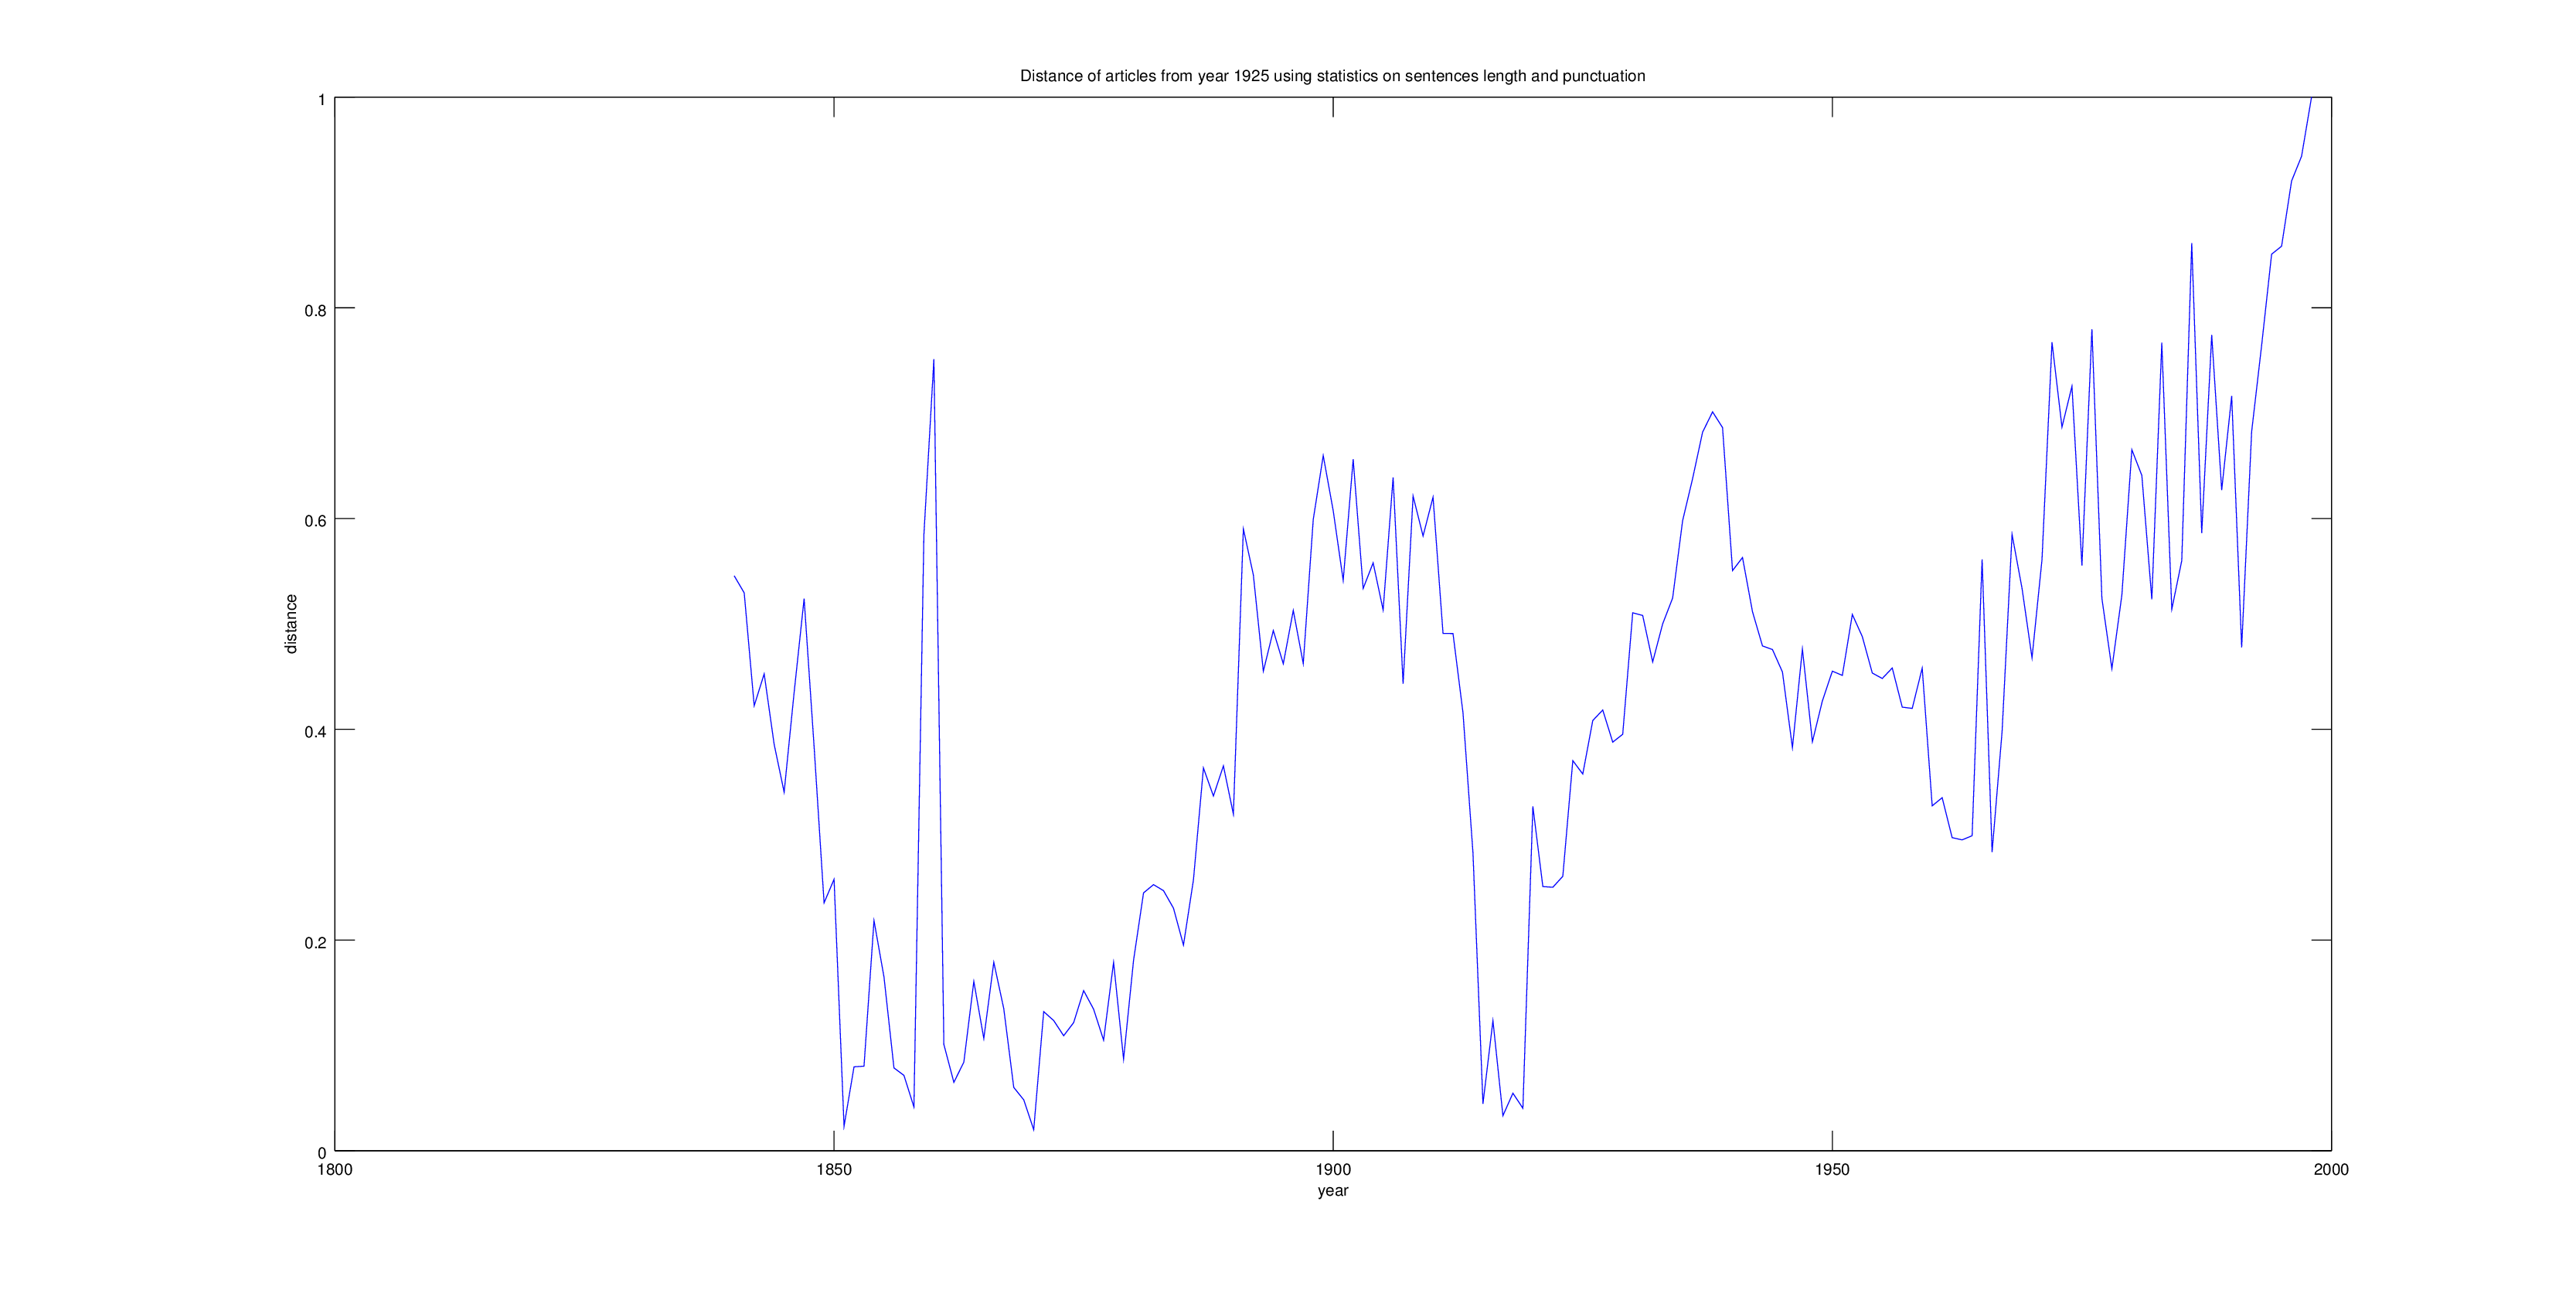
\includegraphics[scale=0.5]{Pictures/date_articles/punctuation/graph.png}
    \caption{Distance between a sample of 15 random articles from 1925 and each year}
    \label{punct_metric_1925}\hfill
\end{figure}

As we can see, it does not work that well, but with more time, we could have used machine learning methods instead of a simple euclidean distance, we think it could be useful to combine the result obtained them with other distances to enhance the classification.

\subsection{Cross Validation}
To have stronger values when we date articles, we wrote a script that runs several times each metrics for a different subsets of article of the same year. The idea here is to have an average on the error of each metric to be able to compare them together. We obtained the following results for random years.\\

\textbf{Mean error for different metrics for 15 articles in year 1843 with 15 iterations}\\
\begin{tabular}{p{3cm} p{5cm}}
Distance1 :& 0\\
Cosine :& 10.73333333333333333333\\
Cosine-TFIDF :& .40000000000000000000\\
Chi-Square :& 112.40000000000000000000\\
Kullback-Leibler :& 11.33333333333333333333\\
OutOfPlace :& 3.00000000000000000000\\
Punctuation :& 33.13333333333333333333\\
\end{tabular}\\
 
\textbf{Mean error for different metrics for 15 articles in year 1854 with 15 iterations}\\
\begin{tabular}{p{3cm} p{5cm}}
    Distance1 :& 8.00000000000000000000\\
    Cosine :& 9.86666666666666666666\\
    Cosine-TFIDF :& 0\\
    Chi-Square :& 111.86666666666666666666\\
    Kullback-Leibler :& 0\\
    OutOfPlace :& 8.00000000000000000000\\
    Punctuation :& 15.80000000000000000000\\
\end{tabular}\\
 
\textbf{Mean error for different metrics for 15 articles in year 1888 with 15 iterations}\\
\begin{tabular}{p{3cm} p{5cm}}
    Distance1 :& 42.00000000000000000000\\
    Cosine :& 15.13333333333333333333\\
    Cosine-TFIDF :& 0\\
    Chi-Square :& 62.40000000000000000000\\
    Kullback-Leibler :& .26666666666666666666\\
    OutOfPlace :& 42.00000000000000000000\\
    Punctuation :& 32.80000000000000000000\\
\end{tabular}\\
 
\textbf{Mean error for different metrics for 15 articles in year 1905 with 15 iterations}\\
\begin{tabular}{p{3cm} p{5cm}}
    Distance1 :& 65.80000000000000000000\\
    Cosine :& 17.13333333333333333333\\
    Cosine-TFIDF :& .06666666666666666666\\
    Chi-Square :& 48.40000000000000000000\\
    Kullback-Leibler :& 3.06666666666666666666\\
    OutOfPlace :& 59.00000000000000000000\\
    Punctuation :& 21.06666666666666666666\\
\end{tabular}\\
 
\textbf{Mean error for different metrics for 15 articles in year 1918 with 15 iterations}\\
\begin{tabular}{p{3cm} p{5cm}}
    Distance1 :& 78.93333333333333333333\\
    Cosine :& 4.73333333333333333333\\
    Cosine-TFIDF :& 0\\
    Chi-Square :& 36.33333333333333333333\\
    Kullback-Leibler :& 2.66666666666666666666\\
    OutOfPlace :& 72.00000000000000000000\\
    Punctuation :& 30.86666666666666666666\\
\end{tabular}\\
 
\textbf{Mean error for different metrics for 15 articles in year 1934 with 15 iterations}\\
\begin{tabular}{p{3cm} p{5cm}}
    Distance1 :& 65.60000000000000000000\\
    Cosine :& 17.46666666666666666666\\
    Cosine-TFIDF :& .80000000000000000000\\
    Chi-Square :& 128.93333333333333333333\\
    Kullback-Leibler :& .33333333333333333333\\
    OutOfPlace :& 88.00000000000000000000\\
    Punctuation :& 37.66666666666666666666\\
\end{tabular}\\
 
\textbf{Mean error for different metrics for 15 articles in year 1954 with 15 iterations}\\
\begin{tabular}{p{3cm} p{5cm}}
    Distance1 :& 44.00000000000000000000\\
    Cosine :& 24.60000000000000000000\\
    Cosine-TFIDF :& 0\\
    Chi-Square :& 0\\
    Kullback-Leibler :& .66666666666666666666\\
    OutOfPlace :& 108.00000000000000000000\\
    Punctuation :& 48.06666666666666666666\\
\end{tabular}\\
 
\textbf{Mean error for different metrics for 15 articles in year 1984 with 15 iterations}\\
\begin{tabular}{p{3cm} p{5cm}}
    Distance1 :& 14.00000000000000000000\\
    Cosine :& 7.20000000000000000000\\
    Cosine-TFIDF :& 1.66666666666666666666\\
    Chi-Square :& 3.73333333333333333333\\
    Kullback-Leibler :& 0\\
    OutOfPlace :& 138.00000000000000000000\\
    Punctuation :& 81.80000000000000000000\\
\end{tabular}\\

We observe that two metrics are in general better than the others. These two metrics are the \emph{Kullback-Leibler} Divergence and the Cosine with TF-IDF. Indeed, as explained in section \ref{metrics}, these two metrics are good and we know why. The other metrics are not so bad, even the basic distance which has surprisingly an error of 0 when dating articles from 1843. We think this distance was just lucky with the subset of articles. TOOOOOOOOOOOOOOOOOOOOOOOOODDDDDDDDDDDDDDDOOOOOOOOOOOOOOOOOOOOOOOOOOOO Indeed, we have run the dating of articles with the same options but with different subsets of articles and we can observe that the basic distance is not anymore equal to 0. For the other metrics, we can observe that they vary depending on the year or certainly on the subset of articles.\\

To judge which metric is the best one, we can simply compute the mean error over all our samples. As it takes a lot of time to compute 15 times each metrics, we can't compute it for each year. Here is the overall mean over all the years we tested :\\

\textbf{Mean error for different metrics for 15 articles in the years selected above with 15 iterations per year}\\
\begin{tabular}{p{3cm} p{5cm}}
    Distance1 :& 39.7875\\
    Cosine :& 13.35875\\
    Cosine-TFIDF :& 0.36675\\
    Chi-Square :& 63.008625\\
    Kullback-Leibler :& 2.292\\
    OutOfPlace :& 64.75\\
    Punctuation :& 37.65025\\
\end{tabular}\\

We can observe that, as expected, Cosine with TF-IDF distance and \emph{Kullback-Leibler} Divergence are the best ones.\\

Finally, we made some tests to compare, for a given year, if the number of selected articles to date changes a lot the results of the metrics. And....